\documentclass[a4paper,11pt,fleqn]{article}%fleqn pour aligner les equations à gauche
\usepackage{/home/rweye/Nextcloud/Documents/Overleaf/Styles/Cours}


\newcommand{\chnum}{Chapitre 1}
\newcommand{\chtitle}{Radioactivité et datation}
\newcommand{\dtype}{Activité 2}


\begin{document}
\maketitle
\noindent \fbox{
	\begin{minipage}{.70\textwidth}
	\textbf{Document 1 : Désintégration radioactives naturelles}\\
	L'être humain est soumis à une radioactivité naturelle provenant à la fois de la Terre et de l'espace. Cette radioactivité naturelle ne représente pas de danger. L’écorce terrestre contient des noyaux radioactifs depuis sa formation. D'autres noyaux radioactifs (comme le carbone 14) sont créés dans l'atmosphère suite à l'arrivée de rayons cosmiques, des particules de très haute énergie en provenance de l'espace.\\
	Les noyaux radioactifs se désintègrent spontanément pour donner des noyaux plus stables en émettant des rayonnements et des particules chargées. La demi-vie est la durée nécessaire pour que la moitié des noyaux d'un échantillon radioactif se soit désintégrée.\\
	Les aliments que nous consommons, l'eau que nous buvons et l'air que nous respirons contiennent des éléments radioactifs. La principale source de radioactivité naturelle est le radon \ce{^{222}Rn}, un gaz contenu dans le sous-sol dont la demi-vie vaut 3,8 jours. Dans certaines conditions, le radon passe dans l'atmosphère et ses produits de désintégration peuvent se déposer dans les poumons.
	\end{minipage}
	\begin{minipage}{.30\textwidth}
	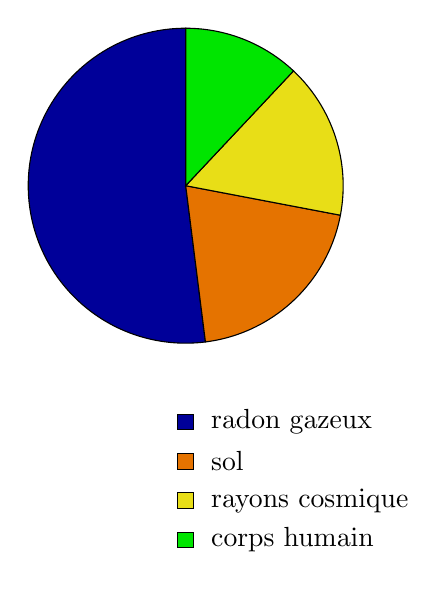
\begin{tikzpicture}
	\draw[fill = blue!60!black] (0,0 ) -- (90:2) arc (90:90+187.2:2) --cycle;
	\draw[fill = orange!90!black] (0,0 ) -- (90+187.2:2) arc (90+187.2:90+259.2:2) --cycle;
	\draw[fill = yellow!90!black] (0,0 ) -- (90+259.2:2) arc (90+259.2:90+316.8:2) --cycle;
	\draw[fill = green!90!black] (0,0 ) -- (90+316.8:2) arc (90+316.8:90+360:2) --cycle;
	\draw[fill = blue!60!black] (-.1,-2.9) rectangle (.1,-3.1);
	\draw[fill = orange!90!black] (-.1,-3.4) rectangle (.1,-3.6);
	\draw[fill = yellow!90!black] (-.1,-3.9) rectangle (.1,-4.1);
	\draw[fill = green!90!black] (-.1,-4.4) rectangle (.1,-4.6);
	\node[right] (H) at (0.2,-3) {radon gazeux};
	\node[right] (H) at (0.2,-3.5) {sol};
	\node[right] (H) at (0.2,-4) {rayons cosmique};
	\node[right] (H) at (0.2,-4.5) {corps humain};
	\end{tikzpicture}
	\end{minipage}
}

\noindent \fbox{
	\begin{minipage}{.60\textwidth}
	\textbf{Document 2 : Le carbone 14 contenu dans les êtres vivants}\\
	Le carbone 14 (\ce{^{14}_{6}C} noté \ce{^{14}C}) est un isotope de l'élément carbone, présent en très faible quantité sur Terre. Il se désintègre naturellement en azote (\ce{^{14}_{7}N}) stable.\\
	Au cours de leurs vie, toue les êtres vivants absorbent du carbone 14 : incorporé par les êtres vivants de la planète lors de la photosynthèse. À leur mort, le carbone 14 qu'ils contiennent n'est plus renouvelé diminue par désintégration radioactive.
	\end{minipage}
	\begin{minipage}{.40\textwidth}
	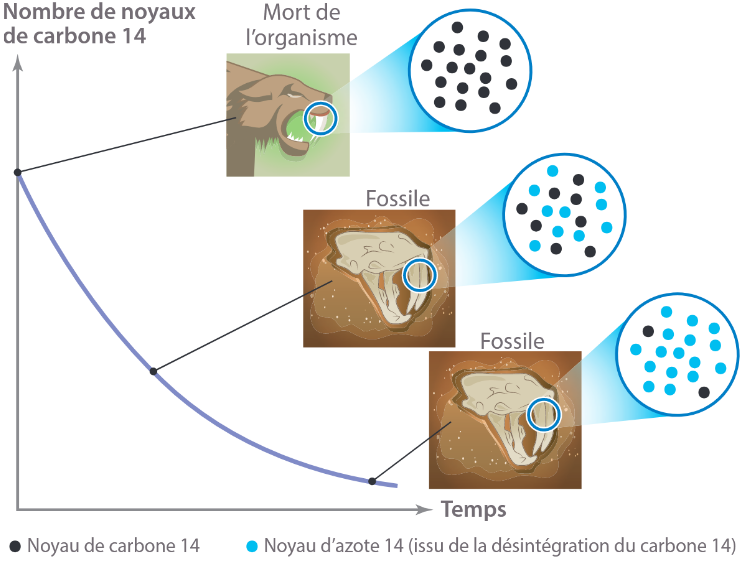
\includegraphics[scale=.3]{Ressources/Act3_Fig1.png}
	\end{minipage}
}

\noindent \fbox{
	\begin{minipage}{.6\textwidth}
	\textbf{Document 3 : Des vestiges que l'on peut dater}\\
	La méthode de datation peur s'appliquer à une multitude de vestiges organiques, humains animaux ou végétaux : peau, os, coquilles, bois ou charbons de bois, plantes, fruits, graines, pollens peuvent être datés. Mais elle peut également être utilisée pour dater des réalisations humaines (tissus, parchemins, poteries, vanneries) : dans ce cas, c'est à partir des matériaux organiques ayant servi à leur fabrication que la datation peut être effectuée.\\
	Le principe est toujours le même : c'est en mesurant la quantité de carbone 14 présent dans un échantillon donné que l'on peut dater la mort de l'organisme.\\
	Par exemple, la datation du charbon de bois présent dans les peintures préhistoriques de la grotte de Niaux  (Ariège) a permis d'affirmer qu'elles ont été dessinées il y a \SI{13000}{ans}.
	\end{minipage}
	\begin{minipage}{.40\textwidth}
	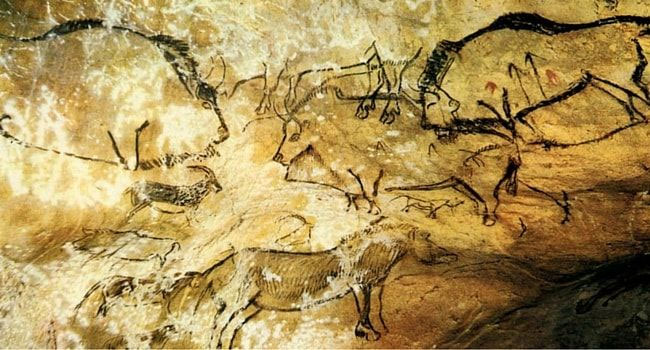
\includegraphics[scale=.32]{Ressources/Act3_Fig2.png}
	\end{minipage}
}

\noindent \fbox{
	\begin{minipage}{.97\textwidth}
	\textbf{Document 4 : L'évolution des techniques de datation}\\
	La datation au carbone 14 a été développée par le physicien et chimiste américain Willard F. Libby (1908-1980). Il effectue la datation de la grotte de Lascaux en 1951 et reçoit en 1960 le prix Nobel de chimie. Les premières datations nécessitaient plusieurs grammes de matières. La détermination des âges était possible dans un domaine compris entre 1000 et 30 000 ans.\\
	Depuis les années 1980, les avancées technologiques ont permis d'utiliser des échantillons de plus en plus petits. Actuellement, on peut remonter sur des périodes comprises entre 300 et 50 000 ans à partir d'\SI{1}{mg} de matière seulement. Au-delà de 50 000 ans, la quantité restante de carbone 14 dans l'échantillon est trop faible pour être mesurée.
	\end{minipage}
}

\noindent \fbox{
	\begin{minipage}{.97\textwidth}
	\textbf{Document 5 : La désintégration nucléaire et la demi-vie}\\
	La désintégration nucléaire est un phénomène spontané et aléatoire : l'instant de désintégration d'un noyau est imprévisible. En revanche, le rythme de désintégration radioactive d'un nombre important de noyau est bien connu. Ce rythme est nommé « demi-vie » et dépend des propriétés radioactives de chaque noyau. La demi-vie $t_{1/2}$ d'un noyau radioactif est la durée au bout de laquelle la moitié des noyaux radioactifs initialement présent dans un échantillon macroscopique s'est désintégrée. Cette durée est caractéristique d'un type de noyau radioactif et peut varier d'une
fraction de seconde à des milliards d'années. Par exemple, le polonium 214 (\ce{^{214}Po} ) a une demi vie de 164 microsecondes contre 4,5 milliards d'années pour l'uranium 238 ( \ce{^{238}U}, principale matière première utilisée dans l'industrie nucléaire).
	\end{minipage}
}

\noindent \fbox{
	\begin{minipage}{.4\textwidth}
	\textbf{Document 6 : Le principe de la lecture de la date de mort}\\
	La datation consiste à comparer la quantité de carbone 14 présent dans un organisme ancien avec celle présente dans un organisme similaire vivant, de même masse. La lecture graphique de la courbe de
décroissance radioactive du carbone 14 permet ainsi d'estimer le temps écoulé depuis la mort de l'organisme.
	\end{minipage}
	\begin{minipage}{.60\textwidth}
	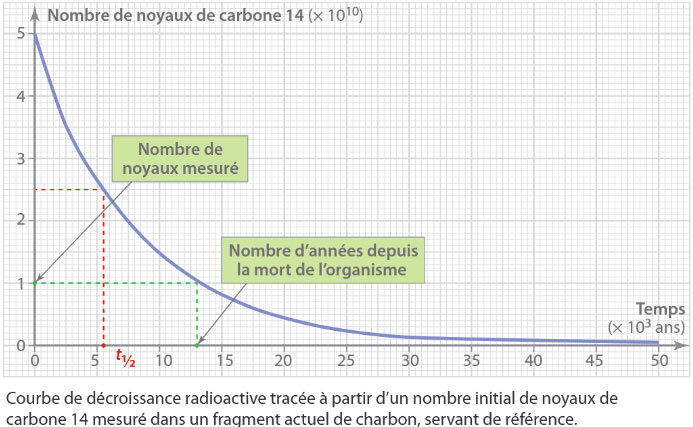
\includegraphics[scale=.45]{Ressources/Act3_Fig3.png}
	\end{minipage}
}

\textbf{Questions :}
\begin{enumerate}
	\item Justifier l'allure de la courbe de décroissance radioactive du \ce{^{14}C}.
	\item A partir de quel moment le nombre d'atomes de \ce{^{14}C} commence t il à diminuer dans un
organisme ?
	\item Qu'appelle-t-on la demi-vie d'un noyau radioactif ? Sachant que $N_0$ est la quantité de noyaux radioactifs présent au départ, montrer qu'à $2 t_{1 /2}$ , le nombre de noyaux restant est $\dfrac{N_0}{4}$. Combien de noyaux reste-t-il à $3t_{1/2}$ ?
	\item Déterminer graphiquement la demi-vie du \ce{^{14}C}.
	\item Déterminer, en détaillant le raisonnement, le nombre de noyaux de \ce{^{14}C} restant dans
l'échantillon de charbon au bout de quatre demi-vies.
	\item Quelle durée sera nécessaire pour obtenir un nombre de noyaux de \ce{^{14}C} égal à \SI{40}{\percent} du nombre initial ?
	\item L'analyse d'un fragment de charbon retrouvé dans la grotte de Lascaux en 1951 a montré qu'il contenait \SI{0,7E10} noyaux de \ce{^{14}C}. Estimer la date d'occupation de la grotte.
\end{enumerate}
\end{document}